\documentclass{article}
\usepackage{tikz}\usetikzlibrary{positioning,arrows.meta}
\begin{document}
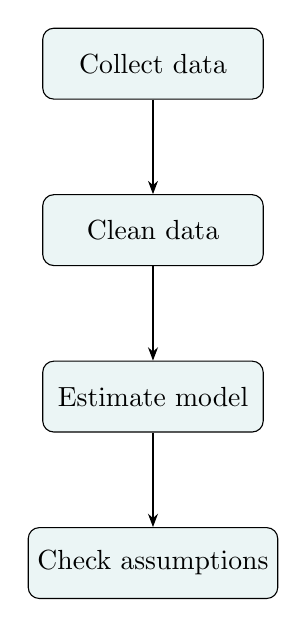
\begin{tikzpicture}[node distance=12mm,>=Stealth,
box/.style={draw,rounded corners,minimum width=28mm,minimum height=9mm,fill=teal!8}]
\node[box] (data){Collect data};
\node[box,below=of data] (clean){Clean data};
\node[box,below=of clean] (estimate){Estimate model};
\node[box,below=of estimate] (check){Check assumptions};
\draw[->] (data)--(clean);\draw[->] (clean)--(estimate);\draw[->] (estimate)--(check);
\end{tikzpicture}
\end{document}
